\documentclass[border=3pt]{standalone}
\usepackage{tikz}
\usetikzlibrary{arrows.meta,calc,positioning}
\tikzset{pin/.style={-{Stealth[length=5pt]}, thick},
  blk/.style={draw, thick, font=\sffamily\small, align=center}}
\begin{document}
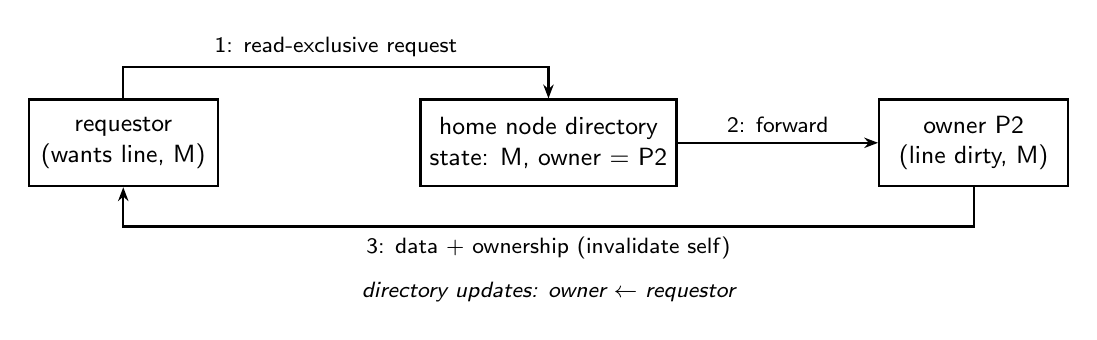
\begin{tikzpicture}[font=\sffamily\small]
  \node[blk, minimum width=24mm, minimum height=11mm] (req) at (0,0) {requestor\\(wants line, M)};
  \node[blk, minimum width=30mm, minimum height=11mm] (dir) at (5.4,0) {home node directory\\state: M, owner = P2};
  \node[blk, minimum width=24mm, minimum height=11mm] (own) at (10.8,0) {owner P2\\(line dirty, M)};
  \draw[pin] (req.north) -- ++(0,4mm) -| node[above, pos=0.25, font=\sffamily\footnotesize]{1: read-exclusive request} (dir.north);
  \draw[pin] (dir.east) -- node[above, font=\sffamily\footnotesize]{2: forward} (own.west);
  \draw[pin] (own.south) -- ++(0,-5mm) -| node[below, pos=0.25, font=\sffamily\footnotesize]{3: data + ownership (invalidate self)} (req.south);
  \node[font=\sffamily\footnotesize\itshape] at (5.4,-1.9) {directory updates: owner $\leftarrow$ requestor};
\end{tikzpicture}
\end{document}
